\documentclass[a4paper, 10pt, conference]{IEEEtran}

%%%%%%%%%%%%%%%%%%%%%%%%%%%%%%%%%%%%%%%%%%%%%%%%%%%%%%%%%%%%%%%%%%%%%%%%%%%%%%%%%%%%%%%%%%%%%%%%%
%
% Packages
%
% Here you can declare the packages you are going to use in your research paper.
% You can also setup the configuration for some of those packages.
%
\usepackage[utf8]{inputenc}
\usepackage[english]{babel}
\usepackage{hyperref}
\usepackage{graphicx}
\usepackage{amsmath}
\usepackage{xcolor}
\usepackage{braket}
%\usepackage{multirow}            % Expands the content of a cell into multiple rows.
%\usepackage{subcaption}          % Adds a separate \caption for each subfigure.
%\usepackage{multicol}            % Expands the content of a cell into multiple columns.

% Color setup for the hyperlinks
\hypersetup{
  colorlinks,
  linkcolor={red!90!black},
  citecolor={green!90!black},
  urlcolor={magenta!90!black}
}
%
%%%%%%%%%%%%%%%%%%%%%%%%%%%%%%%%%%%%%%%%%%%%%%%%%%%%%%%%%%%%%%%%%%%%%%%%%%%%%%%%%%%%%%%%%%%%%%%%%


%%%%%%%%%%%%%%%%%%%%%%%%%%%%%%%%%%%%%%%%%%%%%%%%%%%%%%%%%%%%%%%%%%%%%%%%%%%%%%%%%%%%%%%%%%%%%%%%%
%
% Definitions
%
% Here I introduced some definitions for your research paper.
%
%\addto{\captionsenglish}{\renewcommand{\abstractname}{Summary}}
%
% The following 4 definitions are required by the toy example.
% You can remove/comment them when creating your own research paper.
%
\newcommand{\Prob}[1]{\mathbf{Pr}\left\{ #1 \right\}}
%
%%%%%%%%%%%%%%%%%%%%%%%%%%%%%%%%%%%%%%%%%%%%%%%%%%%%%%%%%%%%%%%%%%%%%%%%%%%%%%%%%%%%%%%%%%%%%%%%%

\begin{document}          % Start of your research paper.


%%%%%%%%%%%%%%%%%%%%%%%%%%%%%%%%%%%%%%%%%%%%%%%%%%%%%%%%%%%%%%%%%%%%%%%%%%%%%%%%%%%%%%%%%%%%%%%%%
%
% Title page
%
% You have to modify this information adapting it to your own research paper. 
%
\title{Quantum Supremacy}
\author{
\IEEEauthorblockN{Student's name}
\IEEEauthorblockA{Amsterdam University of Applied Science\\
Amsterdam, The Netherlands \\
student.email@hva.nl}
}
%
%%%%%%%%%%%%%%%%%%%%%%%%%%%%%%%%%%%%%%%%%%%%%%%%%%%%%%%%%%%%%%%%%%%%%%%%%%%%%%%%%%%%%%%%%%%%%%%%%

\maketitle                % Creates the Title page for your research paper.


%%%%%%%%%%%%%%%%%%%%%%%%%%%%%%%%%%%%%%%%%%%%%%%%%%%%%%%%%%%%%%%%%%%%%%%%%%%%%%%%%%%%%%%%%%%%%%%%%
%
% Abstract
%
% Here you have to write down the Abstract/Summary/Samenvatting of your research paper.
%
\begin{abstract}
The promise of quantum computers is that certain computational tasks might be
executed exponentially faster on a ...
\end{abstract}
%
%%%%%%%%%%%%%%%%%%%%%%%%%%%%%%%%%%%%%%%%%%%%%%%%%%%%%%%%%%%%%%%%%%%%%%%%%%%%%%%%%%%%%%%%%%%%%%%%%


%\clearpage                % Forces LaTeX to produce a page break.
%\tableofcontents          % Creates the Table of Content for your research paper.
%\clearpage                % Forces LaTeX to produce a page break.


%%%%%%%%%%%%%%%%%%%%%%%%%%%%%%%%%%%%%%%%%%%%%%%%%%%%%%%%%%%%%%%%%%%%%%%%%%%%%%%%%%%%%%%%%%%%%%%%%
%
% Sections of the paper
%
% Here you have to introduce every LaTeX file that is part of your research paper.
% Use the \input{•} command to do so. Get used to define each differen section in a
% separate .tex file; for instance, my research paper contains 6 sections therefore 
% I have 6 different files.
%
\section{Introduction}
\label{sec:introduction}
%%%%%%%%%%%%%%%%%%%%%%%%%%%%%%%%%%%%%%%%%%%%%%%%%%%%%%%%%%%%%%%%%%%%%%%%%%%%%%%%%%%%%%%%%%%%%%%%%
%
% The following paragraph contains an example of citation. Use the command (\cite{•}) with
% the appropiate citation identifier. Do not forget to use the parenthesis.
%
%%%%%%%%%%%%%%%%%%%%%%%%%%%%%%%%%%%%%%%%%%%%%%%%%%%%%%%%%%%%%%%%%%%%%%%%%%%%%%%%%%%%%%%%%%%%%%%%%
In the early 1980's, Richard Feynman proposed that a quantum computer would be
an effective tool with which to solve problems in physics and chemistry, given
that it is exponentially costly to simulate large quantum systems with
classical computers (\cite{feynman1982simulating}).

...

...

...

%%%%%%%%%%%%%%%%%%%%%%%%%%%%%%%%%%%%%%%%%%%%%%%%%%%%%%%%%%%%%%%%%%%%%%%%%%%%%%%%%%%%%%%%%%%%%%%%%
%
% This paragraph contains an example of an internal reference. Use the command
% \ref{•} along with the identifier defined with the command \label{•} to create
% a reference to an internal section on your research paper. The label can be
%  defined in any of the .tex files that you have included.
%
%%%%%%%%%%%%%%%%%%%%%%%%%%%%%%%%%%%%%%%%%%%%%%%%%%%%%%%%%%%%%%%%%%%%%%%%%%%%%%%%%%%%%%%%%%%%%%%%%
This research paper is organized as follows. Section~\ref{sec:task} offers
.... Section~\ref{sec:processor} describes the .... Section~\ref{sec:experiments}
reports a .... Finally, in Section~\ref{sec:conclusions} we state ...

\section{What would fit?}
\label{sec:task}
There are plenty of types of quantum computers out there. All with their upsides and downsides. Lets first take a look at what technologies are out there:

\begin{itemize}
  \item Superconducting
  \item Trapped ion
  \item Silicon dot
  \item Photonic
  \item Neutral atoms
  \item NV diamond
\end{itemize}

Where, to be able to fit one of these technologies into a QPU without too many assumptions, it would need to be able to function at room temperature and pressure. The choice already gets limited a lot here, as only NV diamonds can function at room temperature and pressure. This gives us the exact technology to be used for a QPU. 
\\\\
How does it work? The nv diamond quantum computing method is named after the NV diamond faults it uses. An NV fault is a type of fault which can both be naturally present in diamonds or be introduced. Where one carbon is replaced with a nitrogen and another connected carbon is completely removed, creating a vacancy. Which is where it gets its name from, Nitrogen Vacancy diamond faults \cite{wikipedia1}.
\\\\
These faults are then used together with a magnetic field or other method of delivering energy to steer and adjust the faults. So they can be operated on and measured. That being said, there is very little info on how this is done exactly out there, a lot of it is kept behind bars at the moment. So assumptions will have to be made regarding how this is to be controlled and how much voltage a Q-bit will need \cite{article1}.


\begin{figure}
\caption{The layout of a GPU}
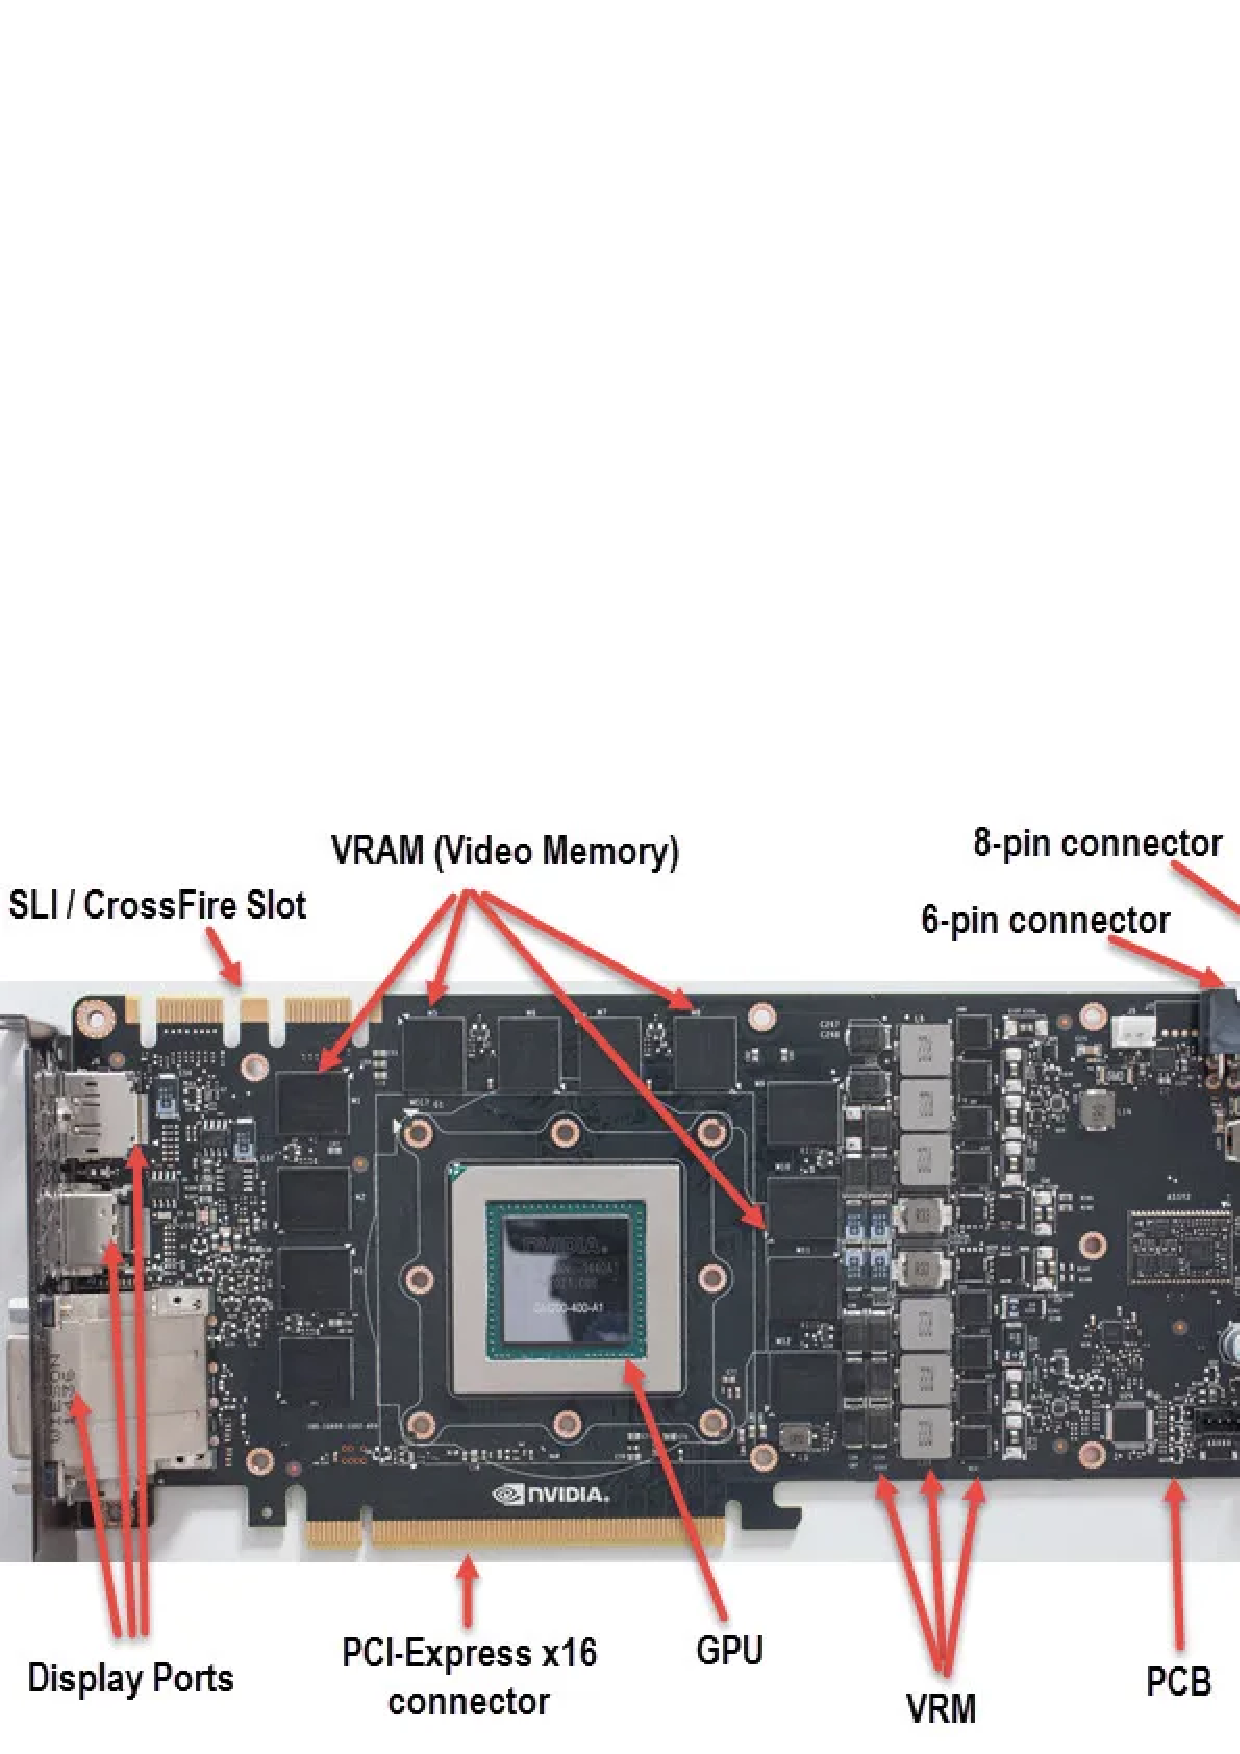
\includegraphics[width = \textwidth]{img/graphics-card-components-3119853491}
\end{figure}

\begin{figure}
\caption{Layout of a GPU chip}
\includegraphics[width = \textwidth]{img/pascal_gp104_block_diagram}
\end{figure}

\section{What do GPU's do?}
\label{sec:processor}
A GPU is used to process a 3D scene into an image which can be displayed to the screen. It gets the vertexes, materials, shaders and all other things which influence the look of a scene and turn it into an image, a frame. It does this 60 times per second most commonly, sometimes even faster if the screen is made for it and the GPU can handle that workload \cite{document1}. 
\\\\
The GPU consists of a couple things, see figure 1 for reference:
\begin{itemize}
	\item a PCIe slot
	\item GPU chip
	\item Display ports
	\item VRAM
	\item a PCB
	\item VRM
	\item x-Pin connectors
\end{itemize}
This list is not exhaustive. but will do for the purposes of explaining how a GPU works. Indeed, the GPU is both the name of the device and the chip on the device. This is due to the trivial name of the device being linked to the most important component. The GPU is a chip which has many smaller sub area's for parallel calculation as can be seen in figure 2, as a scene can contain a lot of objects, pixels and effects. Which can be somewhat calculated in parallel, keep in mind that on stage follows after another. Shaders are done after meshes for example, but multiple meshes can be calculated at the same time \cite{document1}. 
\\\\
The second most important component is VRAM. This is in essence just RAM but is located on the graphics card, which allows it to access this RAM quicker. This ram is used to store the input and output of the GPU. An example of what it would store is: information on the 3D scene and the partially completed image it is rendering. Where the amount of VRAM the card has will affect the complexity the scene may have before the card starts having issues with a bottleneck. 
\\\\
Just to not go on too long, The PCB is the plate all of the components are soldered on. The VRM regulates the voltage going to components, the display port outputs the frames the GPU calculates to a screen. The PCIe slot is where the GPU slots into the motherboard and where it communicates with the CPU. The x-pin connectors describes the amount of pins it needs, the more power a GPU needs the more pins it will require. These pins then connect back to the power supply in a desktop PC. 
\section{Experiments}
\label{sec:experiments}
For the full experiment, we generate quantum circuits using the two--qubit
unitaries measured for each pair during simultaneous operation, rather than a
standard gate for all pairs ...

Finally, we benchmark qubit readout using standard dispersive measurement
~\cite{wallraff2005approaching}. Measurement errors averaged over the $\ket{0}$
and $\ket{1}$ states are shown in Table~\ref{tab:pauli_errors}. We have also
measured the error when operating all qubits simultaneously, by randomly
preparing each qubit in the $\ket{0}$ or $\ket{1}$ state and then measuring all
qubits for the probability of the correct result. We find that simultaneous
readout incurs only a modest increase in per--qubit measurement errors.

%%%%%%%%%%%%%%%%%%%%%%%%%%%%%%%%%%%%%%%%%%%%%%%%%%%%%%%%%%%%%%%%%%%%%%%%%%%%%%%%%%%%%%%%%%%%%%%%%
%
% The following paragraph contains several examples:
%
%   1.- A table. Use the environment \begin{table} ... \end{table} to insert
%       a table.
%
%   2.- Centering in the page. Use the command \centering to center horizontally
%        in the page
%
%   3.- Define and create the table. Use the environment \begin{tabular} ... 
%       \end{tabular} to construct a table. The alignment of the cells is given by
%       the character 'c' and the borders are defined by the character '|'.
%
%   4.- Horizontal line. Use the command \hline to create a horizontal line (border)
%       for the table.
%
%   5.- Table columns and rows. Each column/cell is limited by the character '&" and
%       the rows are limited by the character '\\'
%
%   6.- Change the font color. Use the command \textcolor{color}{text} to apply
%       a given color to the specified text.
%
%   7.- Create a caption for the table. Use the command \caption{•} to include an 
%       explanatory text of the table. Be as self-contained as possible.
%
%   8.- Definition of the label. Use the command \label{•} to be used/referenced in
%       a different section of your research paper.
%
%%%%%%%%%%%%%%%%%%%%%%%%%%%%%%%%%%%%%%%%%%%%%%%%%%%%%%%%%%%%%%%%%%%%%%%%%%%%%%%%%%%%%%%%%%%%%%%%%
\begin{table}[t]
  \centering
  \begin{tabular}{|c|| c | c |}
    \hline
    Average error & Isolated & Simultaneous \\
    \hline
    \hline
    Single--qubit ($e_{1}$) & 0.15\% & 0.16\% \\
    \textcolor{green}{Two--qubit ($e_{2}$)} & \textcolor{green}{0.36\%} & \textcolor{green}{0.62\%} \\
    \textcolor{blue}{Two--qubit, cycle ($e_{2c}$)} & \textcolor{blue}{0.65\%} & \textcolor{blue}{0.93\%} \\
    \textcolor{orange}{Readout ($e_{r}$)} & \textcolor{orange}{3.1\%} & \textcolor{orange}{3.8\%} \\
    \hline
  \end{tabular}
  \caption{Average (mean) values of Pauli errors (black, green, blue) and
           readout errors (orange), measured on qubits in isolation and when
           operating all qubits simultaneously.}
  \label{tab:pauli_errors}
\end{table}
\section{Conclusions}
\label{sec:conclusions}
In conclusion, there are pieces of common software out there which could benefit from a QPU. But, often, this software will already have an acceptable performance. Meaning that it would not be necessary. But one piece of software sticks out, games, it could be very possible that a desktop QPU could improve the performance of games, or in this case, Counter-Strike 2. Which could mean that when a desktop QPU is developed and commercialized, it would become an asset for a new generation of computers.
%
%%%%%%%%%%%%%%%%%%%%%%%%%%%%%%%%%%%%%%%%%%%%%%%%%%%%%%%%%%%%%%%%%%%%%%%%%%%%%%%%%%%%%%%%%%%%%%%%%


%%%%%%%%%%%%%%%%%%%%%%%%%%%%%%%%%%%%%%%%%%%%%%%%%%%%%%%%%%%%%%%%%%%%%%%%%%%%%%%%%%%%%%%%%%%%%%%%%
%
% Bibliography
%
% This command will print the references/bibliography at the end of your research paper.
%
% The bibliography file must follow the bibtex reference format. See the toy example.
%
\bibliographystyle{IEEEtran}
\bibliography{biblio}
%
%%%%%%%%%%%%%%%%%%%%%%%%%%%%%%%%%%%%%%%%%%%%%%%%%%%%%%%%%%%%%%%%%%%%%%%%%%%%%%%%%%%%%%%%%%%%%%%%%


\end{document}          % End of your research paper.
